%************************************************
\chapter{Concept Bottleneck Models}\label{ch:cbm}
%************************************************

Concept Bottleneck Models (CBMs) were first introduced in \cite{koh2020conceptbottleneckmodels} with the idea 
to easily interact with state-of-the-art models using high-level concepts that are understandable for the researchers. 
The general idea is to first predict an intermediate set of human-specified concepts $\mathbf{c}$ based on the input images 
and then use the concepts $\mathbf{c}$ to predict the target label $\mathbf{y}$. The objective is to address three desiderata: 
\cite{margeloiu2021conceptbottleneckmodelslearn}
\begin{itemize}
    \item \textbf{Interpretability}: Being able to note which concepts are important for the targets. 
    \item \textbf{Predictability}: Being able to predict the targets from the concepts alone. 
    \item \textbf{Intervenability}: Being able to replace predicted concept values with ground truth values to improve predictive performance. 
\end{itemize}
These types of models are trained on datapoints $\{(\mathbf{x}^{(i)}, \mathbf{c}^{(i)}, \mathbf{y}^{(i)})\}^n_{i=1}$ where each input $\mathbf{x}$ (usually 
an image $\mathbf{x}\in\mathbb{R}^{H\times W\times C}$) is annotated with the set of concepts $\mathbf{c}\in\mathbb{R}^k$ with $k$ concepts 
and the target $\mathbf{y}\in\mathbb{R}$. We can define the bottleneck model as $f(g(\mathbf{x}))$ where $g: \mathbb{R}^{H\times W\times C} 
\rightarrow \mathbb{R}^k$ maps an input $\mathbf{x}$ into the concept space and then $f: \mathbb{R}^k\rightarrow\mathbb{R}$ maps 
concepts into the target prediction. The bottleneck is performed when the target prediction $\mathbf{\hat y}=f(\mathbf{\hat c})$ relies only 
on the concept predictions $\mathbf{\hat c}=g(\mathbf{x})$ based on the inputs. An illustration of this architecture is shown in Figure \ref{fig:cbm_architecture}. 
For the training of these models, we have three different strategies: 
\begin{itemize}
    \item \textbf{Independent}: learn $\hat f$ and $\hat g$ independently. For $\hat {f} $, minimise the task loss $\mathcal{L}_Y$, 
    which measures the discrepancy between predicted and true targets. Then, for $\hat g$, minimise the concept loss 
    $\mathcal{L}_{C_j}$ for each concept $j$, which measures the discrepancy between predicted and real $j$-th concept. 
    \item \textbf{Sequential}: first learn $\hat g$ and then use the predictions to learn $\hat f$. 
    \item \textbf{Joint}: minimises the weighted sum of both task and concept losses with the hyperparameter $\lambda$, 
    which controls the tradeoff between concept vs. task loss. 
\end{itemize}
One important property of these models is the ability to perform interventions by editing the concept predictions $\hat c$ and 
propagating these changes to the target prediction $\hat y$. This property also makes these models more interpretable in terms 
of high-level concepts since we can see the importance and effect of the inclusion or removal of some concepts for the final 
response. In the original paper, the concept intervention method is applied randomly without any specific criteria or using 
expert knowledge. In a recent paper \cite{shin2022a}, different intervention methods were evaluated to minimise the number of 
concepts to intervene on while maximising task accuracy. The method that achieves the best performance is the one where we 
first intervene on the concepts with the highest predictive uncertainty from the concept predictor $g$, i.e. it first intervenes 
on the concept with the maximum value of $1 / |\hat c_i - 0.5|$. 

\begin{figure}
\centering
\begin{tikzpicture}[
    >=Stealth,
    % Styles
    box/.style={draw=blue!70!black, rectangle, rounded corners, align=center, minimum height=1.5cm, minimum width=3.5cm, fill=blue!5, thick},
    concept/.style={draw=green!70!black, circle, align=center, minimum size=0.8cm, fill=green!5, thick},
    io/.style={align=center, font=\large\bfseries}
    ]

    % 1. Input
    \node (input) [io] {$X$ \\ \normalsize (Input)};

    % 2. Concept Predictor g(x)
    \node (g) [box, below=1.2cm of input] {$g(x)$ \\ \textbf{Concept Predictor} \\ \small (e.g., CNN / Extractor)};

    % 3. Concept Bottleneck
    % Increased spacing below g(x) to give the arrow and 'Predicts' text room to breathe
    \node (c2) [concept, below=2.2cm of g, xshift=-0.5cm] {$c_2$};
    \node (c1) [concept, left=0.4cm of c2] {$c_1$};
    \node (cdots) [right=0.4cm of c2] {$\dots$};
    \node (ck) [concept, right=0.4cm of cdots] {$c_k$};

    % Group the concepts inside a dashed box
    \node[draw=black!60, rectangle, dashed, rounded corners, fit=(c1) (c2) (cdots) (ck), inner sep=0.4cm, thick] (c_box) {};

    % Place the label ON the top border (acting as a title between the arrow and the concepts)
    \node (c_label) [fill=white, font=\bfseries, inner sep=0.15cm] at (c_box.north) {Concept Bottleneck $\mathbf{\hat C}$};

    % 4. Label Predictor f(c)
    \node (f) [box, below=1.5cm of c_box] {$f(\mathbf{c})$ \\ \textbf{Label Predictor} \\ \small (e.g., Linear Model)};

    % 5. Output
    \node (output) [io, below=1.2cm of f] {$\mathbf{\hat Y}$ \\ \normalsize (Prediction)};

    % Connections / Arrows
    \draw[->, thick, draw=black!70] (input) -- (g);
    % Arrow points directly to the top of the new label
    \draw[->, thick, draw=black!70] (g) -- (c_label.north) node[midway, right, font=\small, text=black!70] {Predicts};
    \draw[->, thick, draw=black!70] (c_box.south) -- (f.north);
    \draw[->, thick, draw=black!70] (f.south) -- (output.north) node[midway, right, font=\small, text=black!70] {Predicts};

    % Descriptive Annotations (Anchored to the left)
    \node[left=0.8cm of g, text width=3.2cm, align=right, font=\footnotesize, color=gray!80!black] {Maps raw data to \\ high-dimensional \\ uninterpretable space};
    \node[left=0.8cm of c_box, text width=3.5cm, align=right, font=\footnotesize, color=green!60!black] {Human-understandable \\ concepts \\ (e.g., "has wings")};
    \node[left=0.8cm of f, text width=3.2cm, align=right, font=\footnotesize, color=gray!80!black] {Transparent / simple \\ decision rules based \\ \textbf{only} on concepts};
\end{tikzpicture}
\caption{Architecture of a Concept Bottleneck Model (CBM). The model maps a raw inputs $\mathbf{x}$ to an interpretable intermediate concept space $\mathbf{\hat c}$ before masking the final prediction $\mathbf{\hat y}$.}
\label{fig:cbm_architecture}
\end{figure}

\section{Information Leakage}   
For these types of models, it may often be unrealistic to assume that we will have access to concepts which fully capture the 
relationship between the inputs and targets. Several recent papers have studied the problem of information leakage in these types 
of models based on the previous assumption. This information leakage is usually observed in CBMs trained sequentially or jointly 
\cite{margeloiu2021conceptbottleneckmodelslearn, mahinpei2021promisespitfallsblackboxconcept}, and it appears when the intermediate 
representations encode information that is not present in the concepts $c$, which contains information to predict the final target 
rather than only focusing on getting the concept correct. This leakage has a negative impact on the interpretability and intervenability 
of the model. A CBM model with information leakage may be unsafe for critical decision-making applications, such as clinical scenarios. 
\cite{parisini2026leakageinterpretabilityconceptbasedmodels} We can identify two main types of leakage:   
\begin{itemize}
    \item \textbf{Concept-task leakage}: additional information about the task is stored in the learnt concepts. If concept-task 
    leakage is present, then the learned concept-task mutual information (MI) will be higher than ground-truth concept-task MI. 
    \item \textbf{Interconcept leakage}: additional information about the other concepts is stored in each learned concept. Learned 
    concepts are more predictive of the value of the other learned concepts, resulting in a learned interconcept MI being higher 
    than the ground-truth. 
\end{itemize} 
Several measures of leakage have been proposed in the literature, but none of them has successfully integrated the information-theoretic 
nature of leakage in these types of models. 
\begin{itemize}
    \item \textbf{Concept Performance Metrics}: these are the metrics that indicate the quality of the concept learning, such as for example 
    concept accuracy, precision, recall, F1 score and AUC. These metrics are not sensitive to leakage. Two models can have similar concept 
    performance but have different degrees of information leakage. Concept AUC has more sensitivity in this problem since it contains more 
    information about the concept distribution. 
    \item \textbf{Oracle Impurity Score (OIS)}: this metric was defined in \cite{Espinosa_Zarlenga_2023} to capture leakage. The idea is to 
    train $k(k-1)$ additional simple MLP $\psi_{i,j}$, whose objective is to predict the value of the ground-truth concept $j$ from the 
    learnt representation of concept $i$. This will create the Purity Matrix, defined as $\pi(\hat c, c) = AUC(\psi_{i,j}(\hat c_i), c_j)$. 
    The $(i,j)$-th entry contains the AUC when predicting the ground truth value of concept $j$ given the $i$-th concept representation. 
    The OIS metric is the average difference between the predictivities of learnt and ground truth concepts over pairs of concepts, defined 
    as $$OIS(\hat c, c) = \frac{2}{k} ||\pi(\hat c, c) - \pi(c,c)||_F$$, where the Frobenius norm ensures $0\leq OIS\leq 1$. The value of 
    1 represents a complete misalignment; the $i$-th concept can predict all other concepts except its corresponding one. A value of 0 
    represents a perfect alignment; the $i$-th concept does not encode any unnecessary information for predicting concept $i$. A limitation 
    is the stochasticity of the metric, which involves training neural networks, which is very variable when we evaluate the model several 
    times at test time. 
    \item \textbf{Niche Impurity Score (NIS)}: 
    \item \textbf{Intervention}: the intervention of the predicted concepts with the ground-truth values can be used to evaluate the 
    interpretability and the leakage. A task accuracy that decreases after intervention indicates that the task head expects extra information 
    that is not present in the ground-truth concepts. Models with higher leakage have worse intervention performance. This metric is unable 
    to distinguish between interconcept and concept-task leakage; also, when we have a large number of concepts, the computation is very expensive. 
\end{itemize}




\section{Recent CBMs}  

Concept Embedding Models \cite{zarlenga2022conceptembeddingmodelsaccuracyexplainability} \\
\\
Energy-based Concept Bottleneck Models (ECBMs) \cite{xu2024energybasedconceptbottleneckmodels}

\section{Concept Bottleneck Generative Models}


All the previous models presented in this document are focused on classification or regression problems, which are the original implementations 
of concept bottleneck models. The next step is to combine this idea with generative models to develop a method for interpreting and intervening 
in them, called Concept Bottleneck Generative Models (CBGMs)\cite{ismail2024concept}. This method allows us to steer the generative model, since 
we can change the concept of the image while preserving the image quality, and understand the model by identifying the important concepts that 
are responsible for the output. \\
The general idea is to insert a concept bottleneck (CB) layer into a generative model, which is divided in two parts: the pre-concept bottleneck 
part and the post-concept bottleneck part. The partition depends on the generative model we use (GANs, VAEs, Diffusion). The authors decided to 
use the Concept Embedding framework \cite{zarlenga2022conceptembeddingmodelsaccuracyexplainability} for the concept bottleneck layer and also 
argue that it is unrealistic to expect that the pre-defined human concepts are complete, so they also added a set of unknown concepts that might 
also be required for generation. \\
Each concept is represented with two embeddings: $w_i^+,w_i^- \in \mathbb{R}^m$ representing the active and inactive concept states, respectively. 
The output of the pre-concept bottleneck part of the model, the embedding $h$, is fed into several context networks $\phi$ that map $h$ to the 
two embeddings per concept. Then, a network $\Psi$ is trained to predict the probability of concept $c_i$ from the joint embedding space, 
$\hat c_i = \Psi_i([w_i^+, w_i^-]^T)\in[0,1]$. The final context embedding $w_i$ is defined as a weighted mixture of the two embeddings as 
$w_i=(\hat c_i w_i^+ + (1-\hat c_i)w_i^-)$. All the $k$ concept embeddings are concatenated to obtain the final vector that is fed to the 
post-concept network. For the intervention, we simply have to modify the concept probability $\hat c_i$ to $\bar c_i$ in the weighted mixture of 
$w_i$. A visualization of the concept layer is shown in Figure \ref{fig:cgbm_architecture}.
\begin{figure}
    \centering
    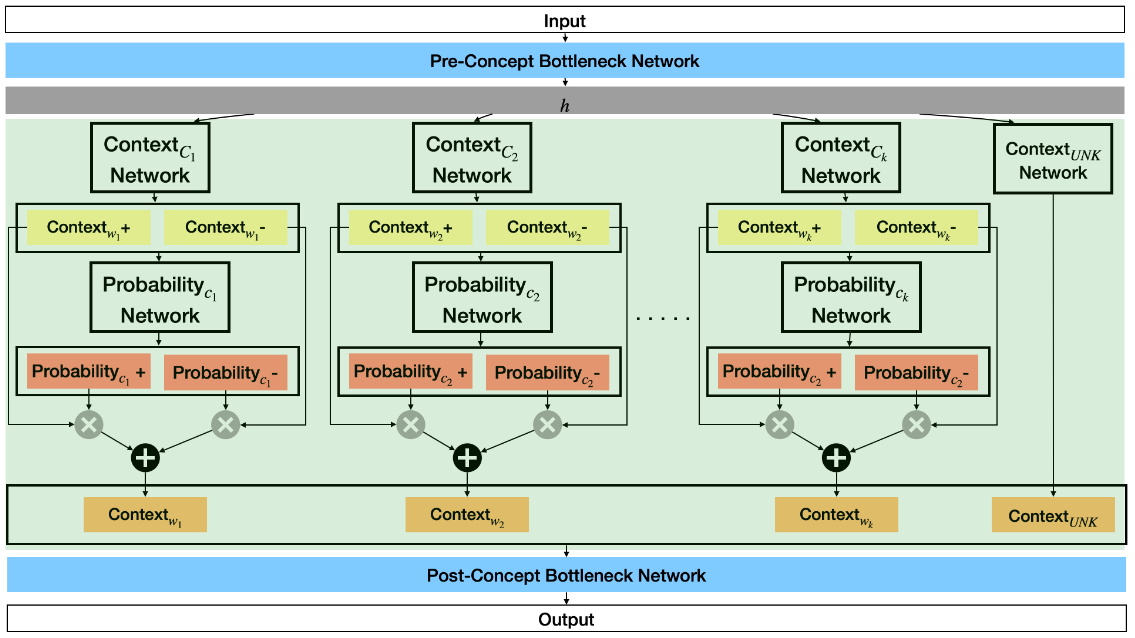
\includegraphics[width=0.9\linewidth]{gfx/cbm/cbgm.png}
    \caption{Architecture of the concept layer in the Concept Bottleneck Generative Model (CBGM) for a generic generative model.}
    \label{fig:cgbm_architecture}
\end{figure}
The loss function is defined as $$\mathcal{L} = \mathcal{L}_{task} + \alpha\mathcal{L}_{con} + \beta\mathcal{L}_{orth},$$ where $\alpha$ and 
$\beta$ are hyperparameters that control the importance of the concept and orthogonality loss, respectively. As we can see, the loss consists 
of three parts: 
\begin{itemize}
    \item \textbf{Task Loss}: the base objective function of the generative model family. 
    \item \textbf{Concept Loss}: is the binary cross-entropy loss between the predicted and real concept probabilities. 
    \item \textbf{Concept Orthogonality Loss}: encourage the unknown concepts to be orthogonal to the outputs of each concept network using an orthogonality constraint defined as: $$\mathcal{L}_{orth} = \sum_{f\in B}\frac{\sum_{i=1}^{i=k}|\langle w_i, w_{k+1} \rangle|}{\sum_{i=1}^{i=k}1},$$ where $\langle \cdot, \cdot \rangle$ is the cosine similarity and $j$ denotes each sample in the mini-batch of size $B$. 
\end{itemize} 
One of the main limitation of the previous method is that the generative model needs to be trained from scratch with the new concept bottleneck 
layer and using a dataset with ground-truth concept annotations. To build a more efficient and scalable method, we can use post-hoc generative 
concept bottleneck models \cite{kulkarni2025interpretablegenerativemodelsposthoc}, which can transform any pre-trained generative model into a 
interpretable one with concept bottleneck layer.  \\
Based on the setup of the previous method, where we divided the generative model in two parts ($g = g_2 \circ g_1$, $\mathbf{z}$ initial noise, 
$\mathbf{x}$ generated sample where $\mathbf{x} = g_2(g_1(\mathbf{z})))$, the idea is to include a concept bottleneck autoencoder. The latent 
space of the autoencoder is the concept prediction $\mathbf{c} = E(g_1(\mathbf{z}))$. This concept prediction is defined using the concept embedding 
framework and also includes a set of unknown concepts to complement the human-defined concepts. Then, the decoder $D$ reconstructs the features from 
the fist part of the generative model ($g_1$) based on the concept prediction $\mathbf{c}$, $\mathbf{w'}=D(\mathbf{c})$, where $\mathbf{w}=g_1(\mathbf{z})$
are the original features. Now we can generate samples from the original image features $\mathbf{w}$ as well as from the reconstructed features $\mathbf{w'}$, 
defined as $\mathbf{x}' = g_2(\mathbf{w'}) = g_2(D \circ E(\mathbf{w}))$.
\begin{figure}
    \centering
    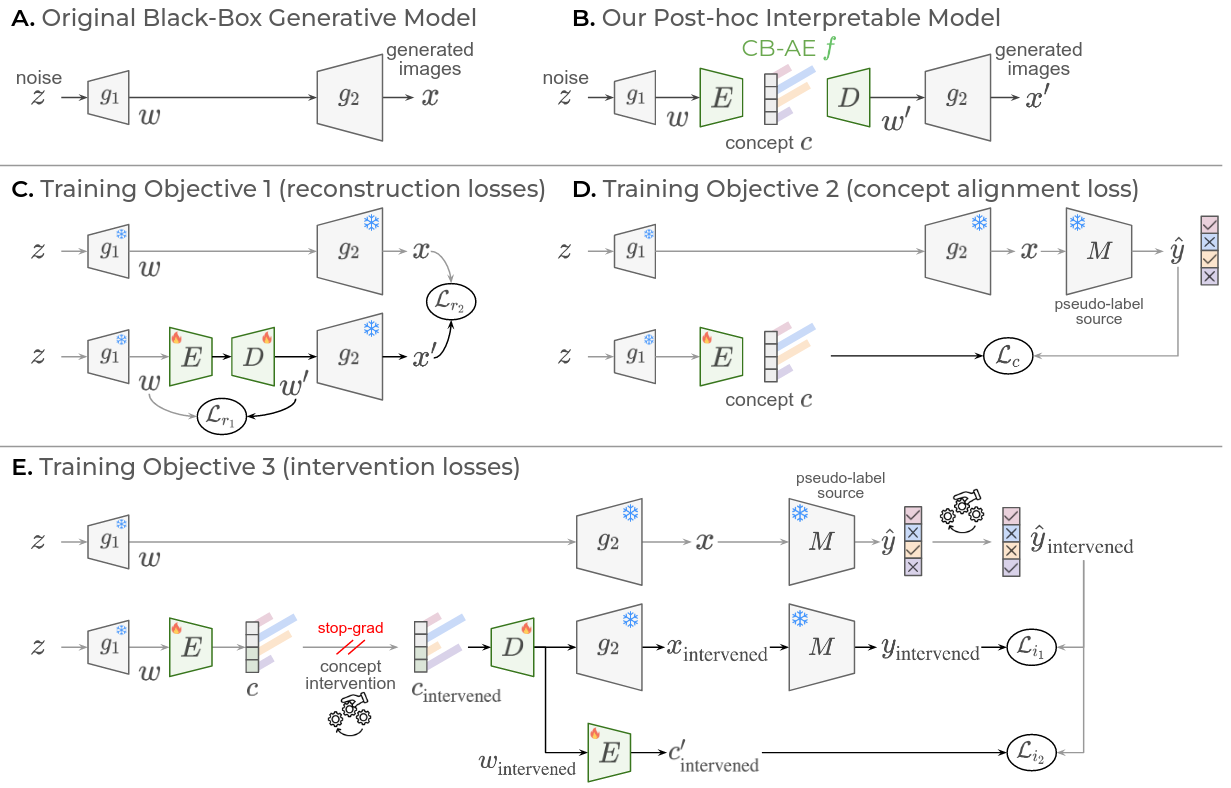
\includegraphics[width=0.9\linewidth]{gfx/cbm/post-hoc_cbgm.png}
    \caption{Architecture of the Post-hoc Concept Bottleneck Generative Model where the different loss functions are illustrated.}
    \label{fig:post_cgbm_architecture}
\end{figure}
For the training of this model, where the generative model is keep frozen, the authors defined three different objective functions based on the different desired goals: 
\begin{itemize}
    \item \textbf{Reconstruction Losses}: we sample $\mathbf{w}$ from the first part of the generative model and use it to generate the original image $\mathbf{x}$. The,
    we introduce $\mathbf{w}$ in the autoencoder to get the reconstructed features $\mathbf{w}'$, which is used to generate the reconstructed image $\mathbf{x}'$. The 
    reconstruction losses are defined as the distance between the original and reconstructed features and images, respectively. The definition is the following: 
    \begin{equation}
        \min_{E,D} \left[ \mathcal{L}_{r_1}(\mathbf{w}, \mathbf{w}') + \mathcal{L}_{r_2}(\mathbf{x}, \mathbf{x}') \right].
    \end{equation}
    \item \textbf{Concept Alignment Loss}: first we have to obtain the pseudo-labels $\mathbf{\hat y} = M(\mathbf{x})$ from a generated image $\mathbf{x}$. This model $M$ can be
    a supervised model or a zero-shot model, such as CLIP. Then, we can obtain the concept prediction $\mathbf{c} = E(g_1(\mathbf{z}))$ and use it to generate the image $\mathbf{x}'$. 
    We can also obtain the pseudo-labels $\mathbf{\hat y'} = M(\mathbf{x}')$ from the generated image. The concept alignment loss is defined as the distance between the pseudo-labels 
    of the original and the predicted concepts. The definition is the following:
    \begin{equation}
        \min_{E} \mathcal{L}_{c}(\mathbf{\hat y}, \mathbf{c}).
    \end{equation}
    \item \textbf{Intervention Losses}: they added a third loss to encourage the steerability of the model, which is an important property of CBMs. The idea is to encourage the decoder 
    $D$ to produce realistic $\mathbf{w'}$ when the concepts are modified. First, we have to select a concept $i$ to intervene by swaaping the logits in the latent concept space to obtain the 
    $\mathbf{c}_{int}$. With the intervened concepts, we can reconstruct the intervened features $\mathbf{w}_{int}$ and the intervened image $\mathbf{x}_{int}$, and using the pseudo-labeler, we can 
    get the concept prediction $\mathbf{y}_{int} = M(\mathbf{x}_{int})$. The final step is to intervene the pseudo-label of the original image by changing only the concept $i$ and get 
    $\mathbf{\hat y}_{int}$. The intervention loss is defined as the distance between the intervened pseudo-labels, which encourages the model to generate images that reflect the concept changes. 
    The definition is the following: 
    \begin{equation}
        \min_{E,D} \mathcal{L}_{i_1}(\mathbf{\hat y}_{int}, \mathbf{y}_{int}).
    \end{equation}
    Also, to improve consistency, they pass the intervened features $\mathbf{w}_{int}$ through the encoder to get the concept predction $\mathbf{c'}_{int}$ and apply cross-entropy loss defined as:
    \begin{equation}
        \min_{E, D} \mathcal{L}_{i_2}(\mathbf{\hat y}_{int}, \mathbf{c'}_{int}).
    \end{equation}
\end{itemize}
The next step is the method called Concept Bottlenecks on Energy Landscapes (CoBEla) \cite{kim2026cobelasteeringtransparentgeneration}, which presents a decoder-free and 
energy-based framework that use a pre-trained frozen generative model. Assume we have the same setup as before, with a generative model divided in two parts and a pseudo-labeler. 
They perturb the intermediate features using the DDPM cosine scheduler to get $\mathbf{w}_t$. For each concept $k$, they define an energy network $E_{\theta}$ that takes as input 
the perturbed features $\mathbf{w}_t$ and the concept $c_k$, which is a learnable concept embedding. The encoder outputs two logits and it is defined as two conditional residual blocks with 
FiLM conditioning \cite{perez2017filmvisualreasoninggeneral}. The concept score is defined as the positive-class probability, which leads to the definition of the interpretable bottleneck score vector
$\mathbf{s} = [s_1, s_2, \ldots, s_K]$. Then, the logits are converted into scalars to represent the energy for each concept, where the aggregation of per-concept energies is defined as 
$\mathcal{E}_{\theta}(\mathbf{w}_t)$, which is used in the score matching loss (defined in Section -- and Equation --) as the noise prediction of the energy-based model. As a complementary loss, 
we have the concept loss that compare the per-concept logits with the pseudo-labels. The total objective is defined as 
\begin{equation}
    \mathcal{L}(\theta) = \lambda_1\mathcal{L}_{score} + \lambda_2\mathcal{L}_{concept}.
\end{equation} 
The visualization of the framework is shown in Figure \ref{fig:cobela_architecture}. 
\begin{figure}
    \centering
    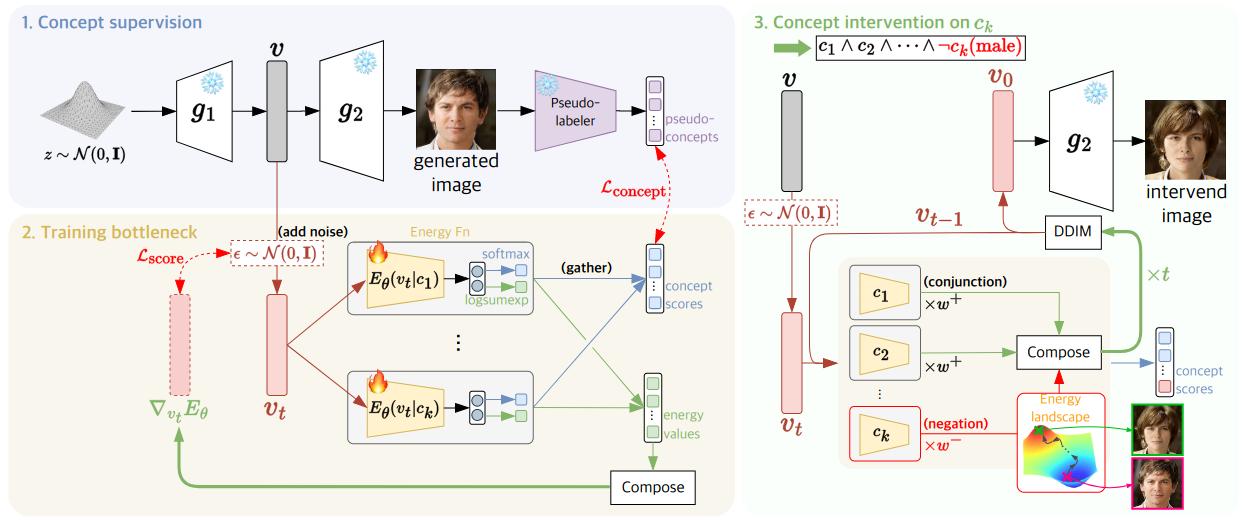
\includegraphics[width=0.9\linewidth]{gfx/cbm/cobela.png}
    \caption{Architecture of the CoBEla Model where the training and guided generation processes are illustrated.}
    \label{fig:cobela_architecture}
\end{figure}
In test time, we assign an intervention weight to each concept that yields to the final weighted energy defined as:
\begin{equation}
    \mathcal{E}_{\theta}(\mathbf{w}_t) = \sum_{k=1}^K \lambda_k E_{\theta}(\mathbf{w}_t, c_k).
\end{equation}
This model allows for the conjunction and negation of concepts, which is a very interesting property that allows for more complex interventions. They used the DDIM sampling method to obtain the final 
generated intermediate features using the weighted energy, which is then fed to the second part of the generative model to get the final generated image.


%*****************************************
%*****************************************
%*****************************************
%*****************************************
%*****************************************